\chapter{Manuel d'Utilisation}

\section{Introduction à l'Application}

Ce chapitre présente un guide détaillé d'utilisation de l'application d'enchères automobiles, destiné aux différents utilisateurs du système. L'application permet de participer à des enchères de véhicules en temps réel, de suivre les enchères en cours, et de gérer son profil utilisateur.

\subsection{Public Cible}

L'application s'adresse à deux catégories principales d'utilisateurs:

\begin{description}
    \item[Utilisateurs Standard] Personnes intéressées par l'achat de véhicules via le système d'enchères. Ces utilisateurs peuvent consulter les enchères disponibles, placer des enchères, et suivre leurs activités.
    \item[Administrateurs] Gestionnaires de la plateforme responsables de la configuration des enchères, de l'ajout des véhicules, et de la gestion des utilisateurs.
\end{description}

\subsection{Prérequis Techniques}

Pour utiliser l'application, les conditions suivantes sont nécessaires:

\begin{itemize}
    \item Un smartphone sous iOS (version 12 ou supérieure) ou Android (version 8 ou supérieure)
    \item Une connexion internet stable (Wi-Fi ou données mobiles)
    \item Un espace de stockage minimal de 100 Mo sur l'appareil
    \item Un compte email valide pour l'inscription
\end{itemize}

\section{Installation et Configuration}

\subsection{Téléchargement de l'Application}

L'application peut être téléchargée depuis les plateformes officielles:

\begin{itemize}
    \item \textbf{iOS}: App Store
    \item \textbf{Android}: Google Play Store
\end{itemize}

La recherche peut être effectuée avec les mots-clés "Car Auction App" ou en scannant le QR code disponible sur le site web officiel.

\subsection{Création de Compte}

Pour utiliser l'application, un compte utilisateur est nécessaire:

\begin{enumerate}
    \item Ouvrir l'application après installation
    \item Sélectionner l'option "S'inscrire"
    \item Remplir le formulaire d'inscription avec:
    \begin{itemize}
        \item Nom d'utilisateur
        \item Adresse email
        \item Mot de passe (au moins 8 caractères, incluant lettres, chiffres et caractères spéciaux)
        \item Informations de profil optionnelles
    \end{itemize}
    \item Accepter les conditions d'utilisation
    \item Cliquer sur "Créer un compte"
    \item Vérifier l'email de confirmation reçu et suivre les instructions
\end{enumerate}

\subsection{Connexion}

Une fois le compte créé, la connexion s'effectue comme suit:

\begin{enumerate}
    \item Ouvrir l'application
    \item Saisir l'email et le mot de passe
    \item Sélectionner "Se souvenir de moi" (optionnel)
    \item Appuyer sur "Se connecter"
\end{enumerate}

En cas d'oubli du mot de passe, l'option "Mot de passe oublié" permet de recevoir un email de réinitialisation.

\section{Interface Utilisateur}

\subsection{Navigation Principale}

L'interface de l'application est organisée autour de cinq sections principales accessibles via la barre de navigation inférieure:

\begin{description}
    \item[Accueil] Affiche les enchères en vedette et les annonces importantes
    \item[Enchères] Liste toutes les enchères disponibles avec options de filtrage
    \item[Mes Enchères] Suivi des enchères auxquelles l'utilisateur participe
    \item[Notifications] Centre de notifications pour les alertes et mises à jour
    \item[Profil] Gestion des informations personnelles et préférences
\end{description}

\begin{figure}[h]
    \centering
    % Placeholder pour une image de l'interface - à remplacer par une capture d'écran réelle
    % \includegraphics[width=0.7\textwidth]{images/interface_navigation.png}
    \caption{Navigation principale de l'application}
    \label{fig:nav-principale}
\end{figure}

\subsection{Écran d'Accueil}

L'écran d'accueil présente:

\begin{itemize}
    \item Un carrousel des enchères populaires ou se terminant bientôt
    \item Des statistiques sur le marché (nombre d'enchères actives, etc.)
    \item Un accès rapide aux dernières enchères consultées
    \item Les actualités et annonces de la plateforme
\end{itemize}

\section{Participation aux Enchères}

\subsection{Recherche et Consultation des Enchères}

Pour trouver des véhicules:

\begin{enumerate}
    \item Accéder à l'onglet "Enchères"
    \item Utiliser la barre de recherche pour des mots-clés spécifiques
    \item Appliquer des filtres selon:
    \begin{itemize}
        \item Marque et modèle
        \item Année de fabrication
        \item Prix (fourchette)
        \item Kilométrage
        \item Type de carburant
        \item Statut de l'enchère (à venir, en cours, terminée)
    \end{itemize}
    \item Trier les résultats par prix, popularité ou date de fin
    \item Sélectionner un véhicule pour afficher sa fiche détaillée
\end{enumerate}

\subsection{Détails d'une Enchère}

La fiche détaillée d'un véhicule comprend:

\begin{itemize}
    \item Galerie d'images du véhicule
    \item Informations techniques (marque, modèle, année, kilométrage, etc.)
    \item Description et état du véhicule
    \item Historique d'entretien (si disponible)
    \item Prix actuel et historique des enchères
    \item Nombre d'enchérisseurs
    \item Temps restant avant la fin de l'enchère
    \item Bouton pour placer une enchère
\end{itemize}

\subsection{Placement d'une Enchère}

Pour participer à une enchère:

\begin{enumerate}
    \item Sur la fiche détaillée du véhicule, appuyer sur "Placer une enchère"
    \item Saisir le montant proposé (doit être supérieur au prix actuel)
    \item Vérifier les informations et confirmer
    \item Attendre la confirmation que l'enchère a été acceptée
\end{enumerate}

\begin{figure}[h]
    \centering
    % Placeholder pour une image de l'interface d'enchère - à remplacer par une capture d'écran réelle
    % \includegraphics[width=0.7\textwidth]{images/interface_enchere.png}
    \caption{Interface de placement d'enchère}
    \label{fig:interface-enchere}
\end{figure}

\subsection{Suivi des Enchères}

Pour suivre les enchères auxquelles l'utilisateur participe:

\begin{enumerate}
    \item Accéder à l'onglet "Mes Enchères"
    \item Visualiser les enchères actives, remportées et perdues
    \item Sélectionner une enchère pour:
    \begin{itemize}
        \item Consulter son statut actuel
        \item Voir l'historique des enchères placées
        \item Recevoir des notifications pour cette enchère
        \item Placer une nouvelle enchère (si active)
    \end{itemize}
\end{enumerate}

\section{Gestion du Profil Utilisateur}

\subsection{Modification des Informations Personnelles}

Pour mettre à jour son profil:

\begin{enumerate}
    \item Accéder à l'onglet "Profil"
    \item Sélectionner "Modifier le profil"
    \item Mettre à jour les informations souhaitées:
    \begin{itemize}
        \item Photo de profil
        \item Nom d'utilisateur
        \item Coordonnées (téléphone, adresse)
        \item Préférences de notification
    \end{itemize}
    \item Enregistrer les modifications
\end{enumerate}

\subsection{Gestion des Notifications}

Pour configurer les notifications:

\begin{enumerate}
    \item Accéder à l'onglet "Profil"
    \item Sélectionner "Paramètres de notification"
    \item Activer/désactiver les types de notifications:
    \begin{itemize}
        \item Surenchère sur un véhicule
        \item Rappel de fin d'enchère proche
        \item Enchère remportée/perdue
        \item Nouvelles enchères correspondant aux préférences
        \item Annonces système
    \end{itemize}
    \item Choisir le mode de notification (push, email, ou les deux)
\end{enumerate}

\subsection{Historique des Transactions}

Pour consulter l'historique:

\begin{enumerate}
    \item Accéder à l'onglet "Profil"
    \item Sélectionner "Historique des transactions"
    \item Visualiser:
    \begin{itemize}
        \item Enchères remportées
        \item Paiements effectués
        \item Factures et documents associés
    \end{itemize}
\end{enumerate}

\section{Fonctionnalités Administrateur}

Cette section concerne uniquement les utilisateurs disposant des droits d'administration.

\subsection{Gestion des Véhicules}

Les administrateurs peuvent gérer les véhicules:

\begin{enumerate}
    \item Accéder au panneau d'administration
    \item Sélectionner "Gestion des véhicules"
    \item Pour ajouter un véhicule:
    \begin{itemize}
        \item Cliquer sur "Ajouter un véhicule"
        \item Remplir les informations détaillées
        \item Ajouter des images (minimum 3, maximum 10)
        \item Enregistrer le véhicule
    \end{itemize}
    \item Pour modifier un véhicule:
    \begin{itemize}
        \item Rechercher et sélectionner le véhicule
        \item Modifier les informations nécessaires
        \item Enregistrer les modifications
    \end{itemize}
    \item Pour supprimer un véhicule:
    \begin{itemize}
        \item Rechercher et sélectionner le véhicule
        \item Confirmer la suppression
    \end{itemize}
\end{enumerate}

\subsection{Création et Gestion des Enchères}

Pour gérer les enchères:

\begin{enumerate}
    \item Accéder au panneau d'administration
    \item Sélectionner "Gestion des enchères"
    \item Pour créer une enchère:
    \begin{itemize}
        \item Cliquer sur "Créer une enchère"
        \item Sélectionner le véhicule concerné
        \item Définir le prix de départ
        \item Configurer la date et l'heure de début/fin
        \item Définir les incréments minimaux
        \item Activer/désactiver les fonctionnalités spéciales
        \item Publier l'enchère
    \end{itemize}
    \item Pour gérer une enchère existante:
    \begin{itemize}
        \item Rechercher et sélectionner l'enchère
        \item Modifier les paramètres (si l'enchère n'a pas commencé)
        \item Surveiller l'activité en temps réel
        \item Intervenir en cas de problème (suspension, annulation)
    \end{itemize}
\end{enumerate}

\subsection{Gestion des Utilisateurs}

Pour administrer les comptes utilisateurs:

\begin{enumerate}
    \item Accéder au panneau d'administration
    \item Sélectionner "Gestion des utilisateurs"
    \item Rechercher un utilisateur par nom, email ou ID
    \item Visualiser les informations complètes du compte
    \item Actions possibles:
    \begin{itemize}
        \item Modifier les détails du compte
        \item Réinitialiser le mot de passe
        \item Suspendre/réactiver un compte
        \item Attribuer des droits d'administration
        \item Consulter l'historique d'activité
    \end{itemize}
\end{enumerate}

\section{Résolution des Problèmes Courants}

\subsection{Problèmes de Connexion}

\begin{itemize}
    \item \textbf{Identifiants refusés}: Vérifier l'orthographe, utiliser "Mot de passe oublié"
    \item \textbf{Compte bloqué}: Contacter le support après plusieurs tentatives échouées
    \item \textbf{Erreur de connexion}: Vérifier la connexion internet, redémarrer l'application
\end{itemize}

\subsection{Problèmes avec les Enchères}

\begin{itemize}
    \item \textbf{Enchère refusée}: Vérifier que le montant est supérieur au prix actuel et respecte l'incrément minimal
    \item \textbf{Enchère non enregistrée}: Rafraîchir la page, vérifier la connexion
    \item \textbf{Retard dans les mises à jour}: Fermer et rouvrir l'application pour rétablir la connexion Socket.io
\end{itemize}

\subsection{Problèmes Techniques Généraux}

\begin{itemize}
    \item \textbf{Application lente}: Libérer de l'espace sur l'appareil, fermer les applications en arrière-plan
    \item \textbf{Plantages}: Mettre à jour l'application, redémarrer l'appareil
    \item \textbf{Images non chargées}: Vérifier la connexion, patienter ou rafraîchir
\end{itemize}

\section{Support et Assistance}

\subsection{Centre d'Aide}

Un centre d'aide est accessible depuis l'application:

\begin{enumerate}
    \item Accéder à l'onglet "Profil"
    \item Sélectionner "Aide et support"
    \item Consulter les articles d'aide classés par catégorie
    \item Utiliser la recherche pour trouver des réponses spécifiques
\end{enumerate}

\subsection{Contact du Support}

Pour contacter l'équipe d'assistance:

\begin{enumerate}
    \item Accéder à l'onglet "Profil"
    \item Sélectionner "Aide et support"
    \item Choisir "Contacter le support"
    \item Sélectionner le type de problème
    \item Décrire le problème rencontré
    \item Joindre des captures d'écran si nécessaire
    \item Soumettre la demande
\end{enumerate}

Le délai de réponse habituel est de 24 à 48 heures ouvrables.

\section{Interface de l'Application}

L'application de vente aux enchères d'automobiles offre une interface utilisateur intuitive et conviviale, conçue pour faciliter la participation aux enchères automobiles. Voici les principales fonctionnalités et écrans de l'application :

\subsection{Authentification et Inscription}

\begin{figure}[H]
    \centering
    \begin{subfigure}[b]{0.48\textwidth}
        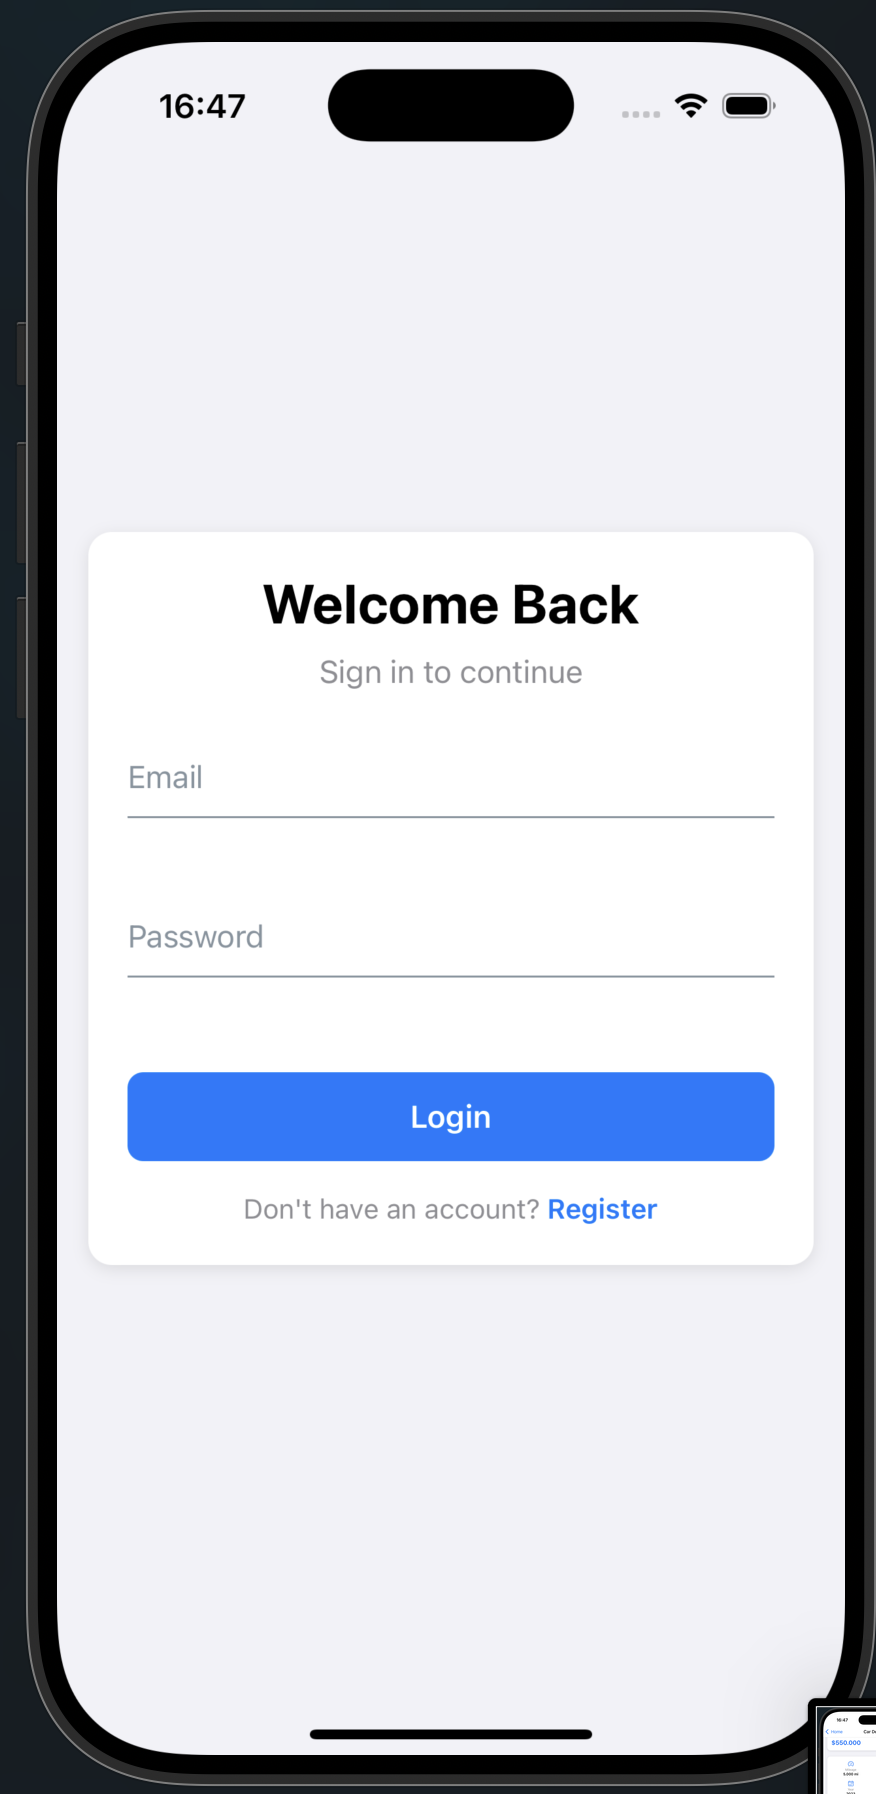
\includegraphics[width=\textwidth]{images/login page.png}
        \caption{Écran de connexion}
        \label{fig:login}
    \end{subfigure}
    \hfill
    \begin{subfigure}[b]{0.48\textwidth}
        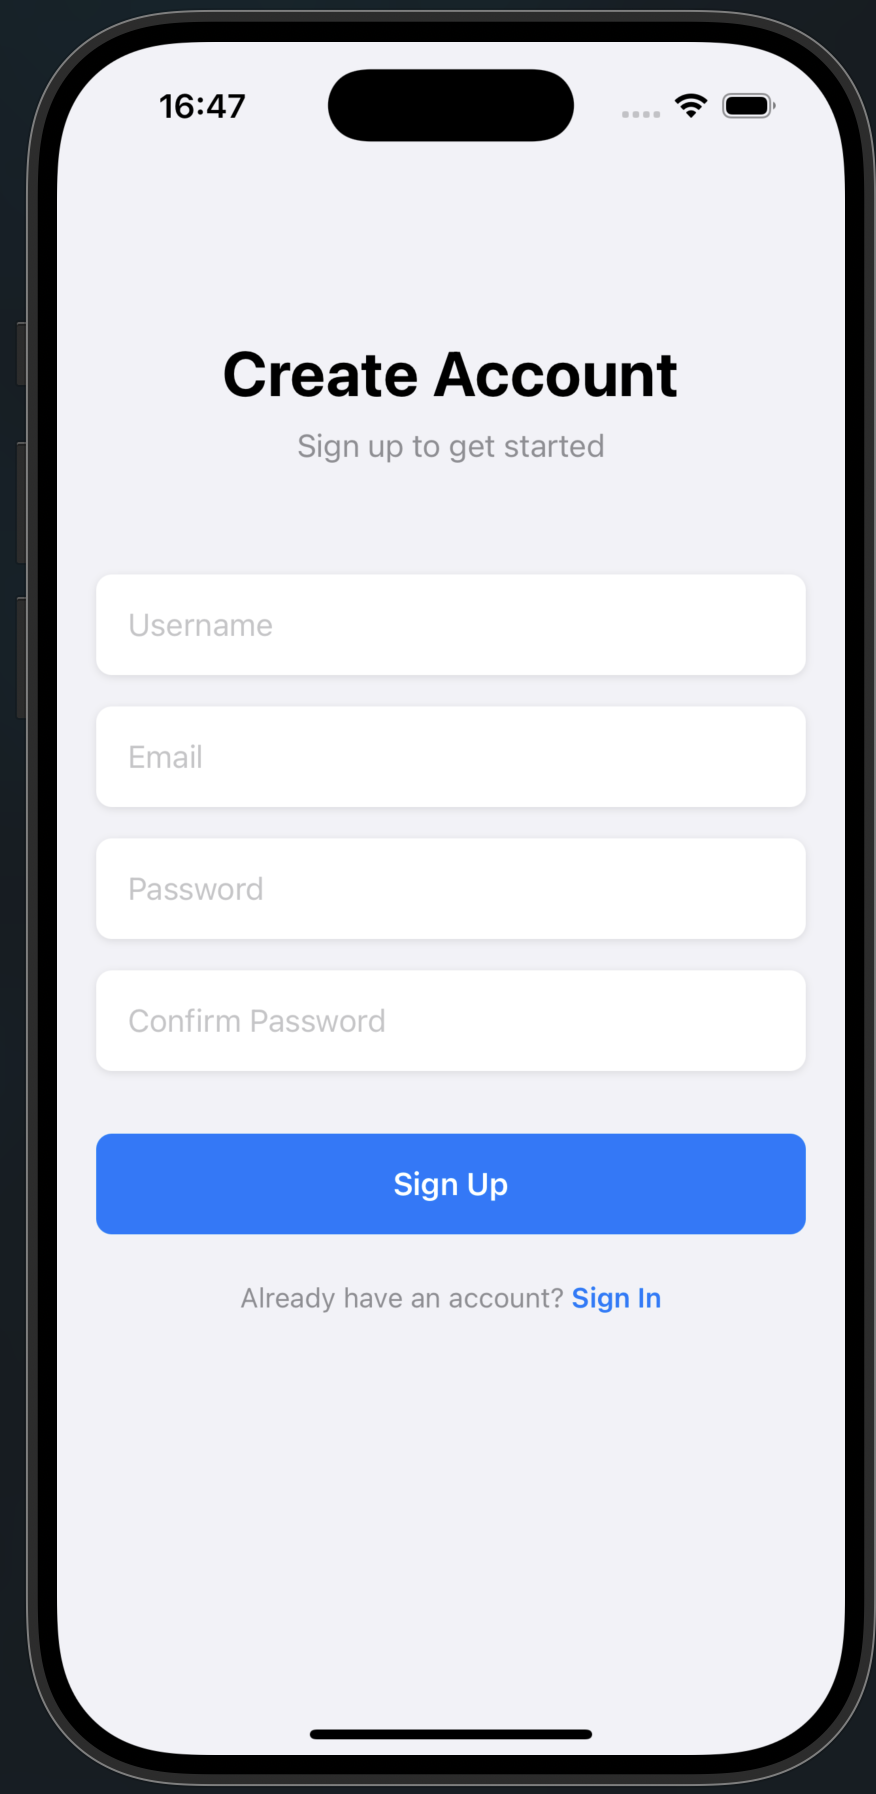
\includegraphics[width=\textwidth]{images/signup page.png}
        \caption{Écran d'inscription}
        \label{fig:register}
    \end{subfigure}
    \caption{Écrans d'authentification de l'application}
    \label{fig:auth-screens}
\end{figure}

L'utilisateur peut accéder à l'application via la page de connexion (Figure \ref{fig:login}) ou créer un nouveau compte via la page d'inscription (Figure \ref{fig:register}). Ces écrans permettent une entrée sécurisée dans le système.

\subsection{Page d'Accueil et Enchères}

\begin{figure}[H]
    \centering
    \begin{subfigure}[b]{0.48\textwidth}
        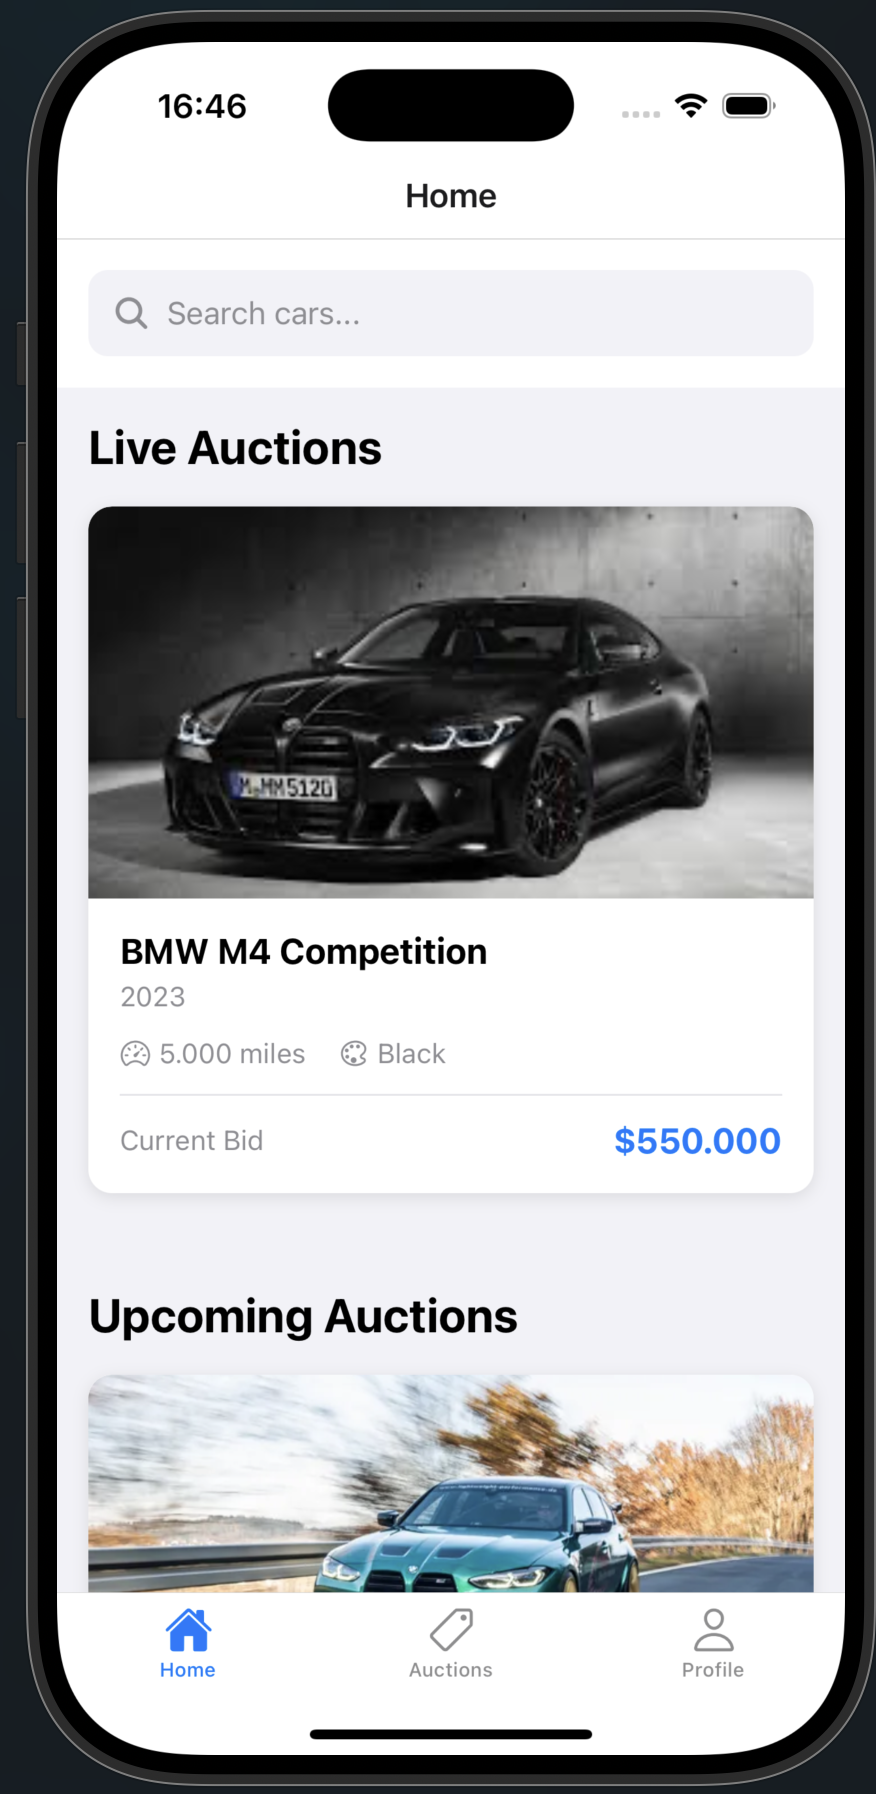
\includegraphics[width=\textwidth]{images/home page with live auctions.png}
        \caption{Enchères en cours}
        \label{fig:home-live}
    \end{subfigure}
    \hfill
    \begin{subfigure}[b]{0.48\textwidth}
        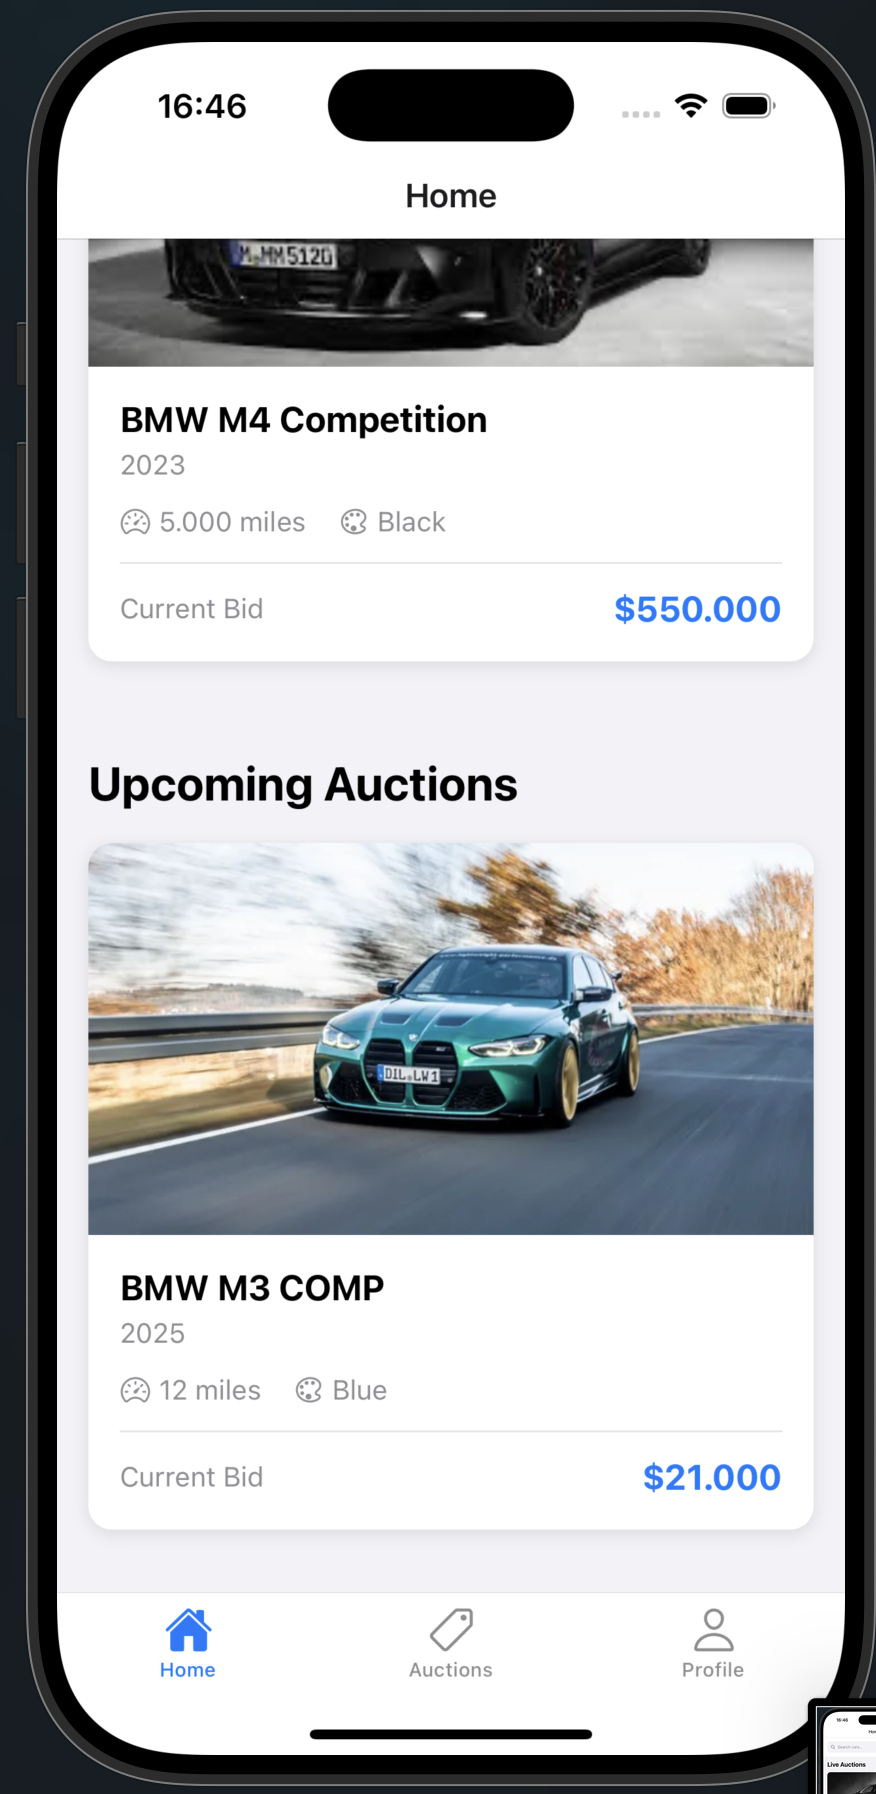
\includegraphics[width=\textwidth]{images/home page with upcoming auctions.png}
        \caption{Enchères à venir}
        \label{fig:home-upcoming}
    \end{subfigure}
    \caption{Pages d'accueil avec différentes vues des enchères}
    \label{fig:home}
\end{figure}

La page d'accueil présente les enchères en cours (Figure \ref{fig:home-live}) et les enchères à venir (Figure \ref{fig:home-upcoming}), permettant aux utilisateurs de parcourir facilement les véhicules disponibles. On y trouve des informations essentielles comme la marque, le modèle, l'année, le kilométrage et le prix actuel de l'enchère.

\subsection{Gestion des Enchères}

\begin{figure}[H]
    \centering
    \begin{subfigure}[b]{0.32\textwidth}
        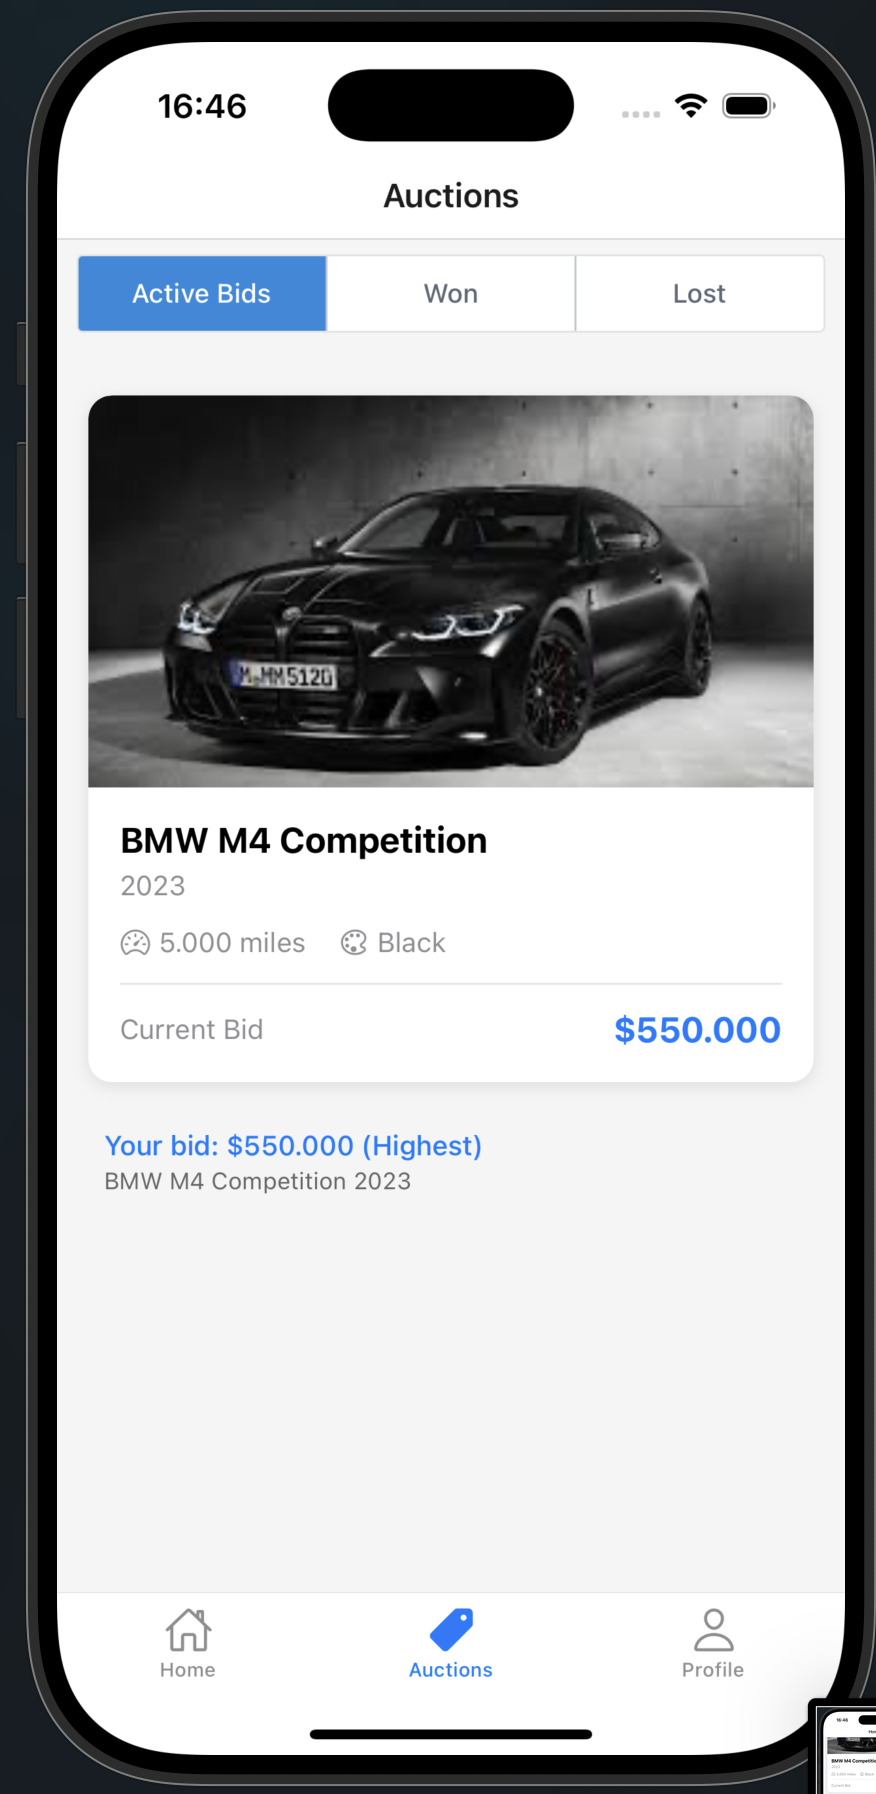
\includegraphics[width=\textwidth]{images/auction page with active bids.png}
        \caption{Enchères actives}
        \label{fig:active-bids}
    \end{subfigure}
    \hfill
    \begin{subfigure}[b]{0.32\textwidth}
        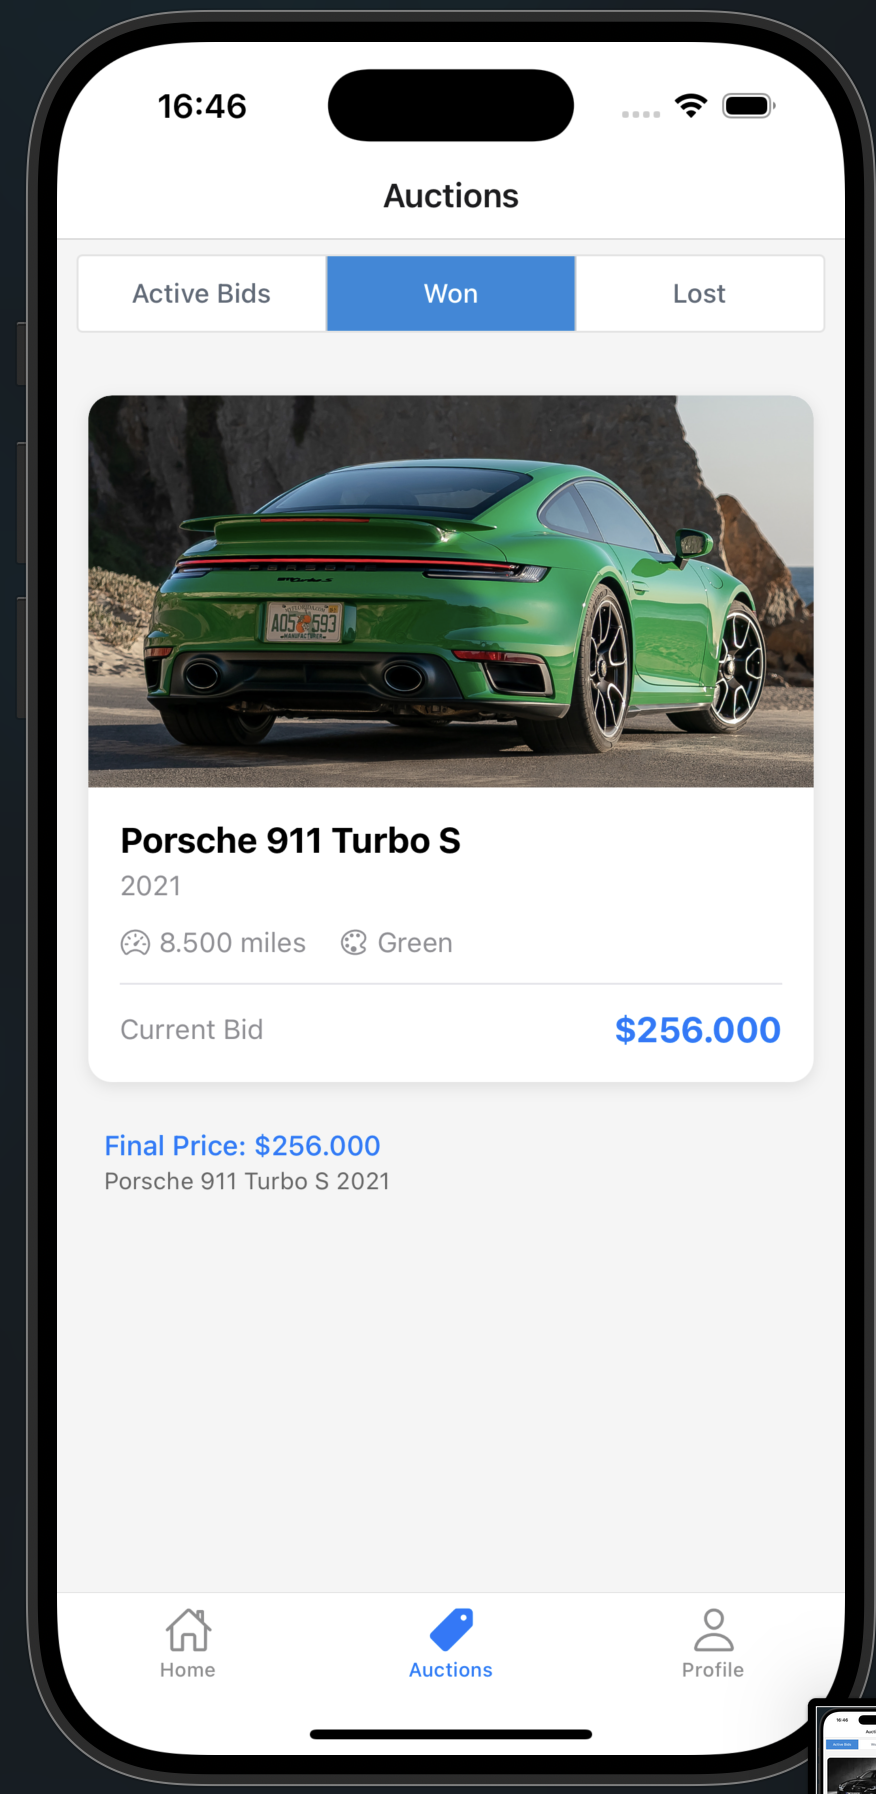
\includegraphics[width=\textwidth]{images/auction page with won bids.png}
        \caption{Enchères gagnées}
        \label{fig:won-auctions}
    \end{subfigure}
    \hfill
    \begin{subfigure}[b]{0.32\textwidth}
        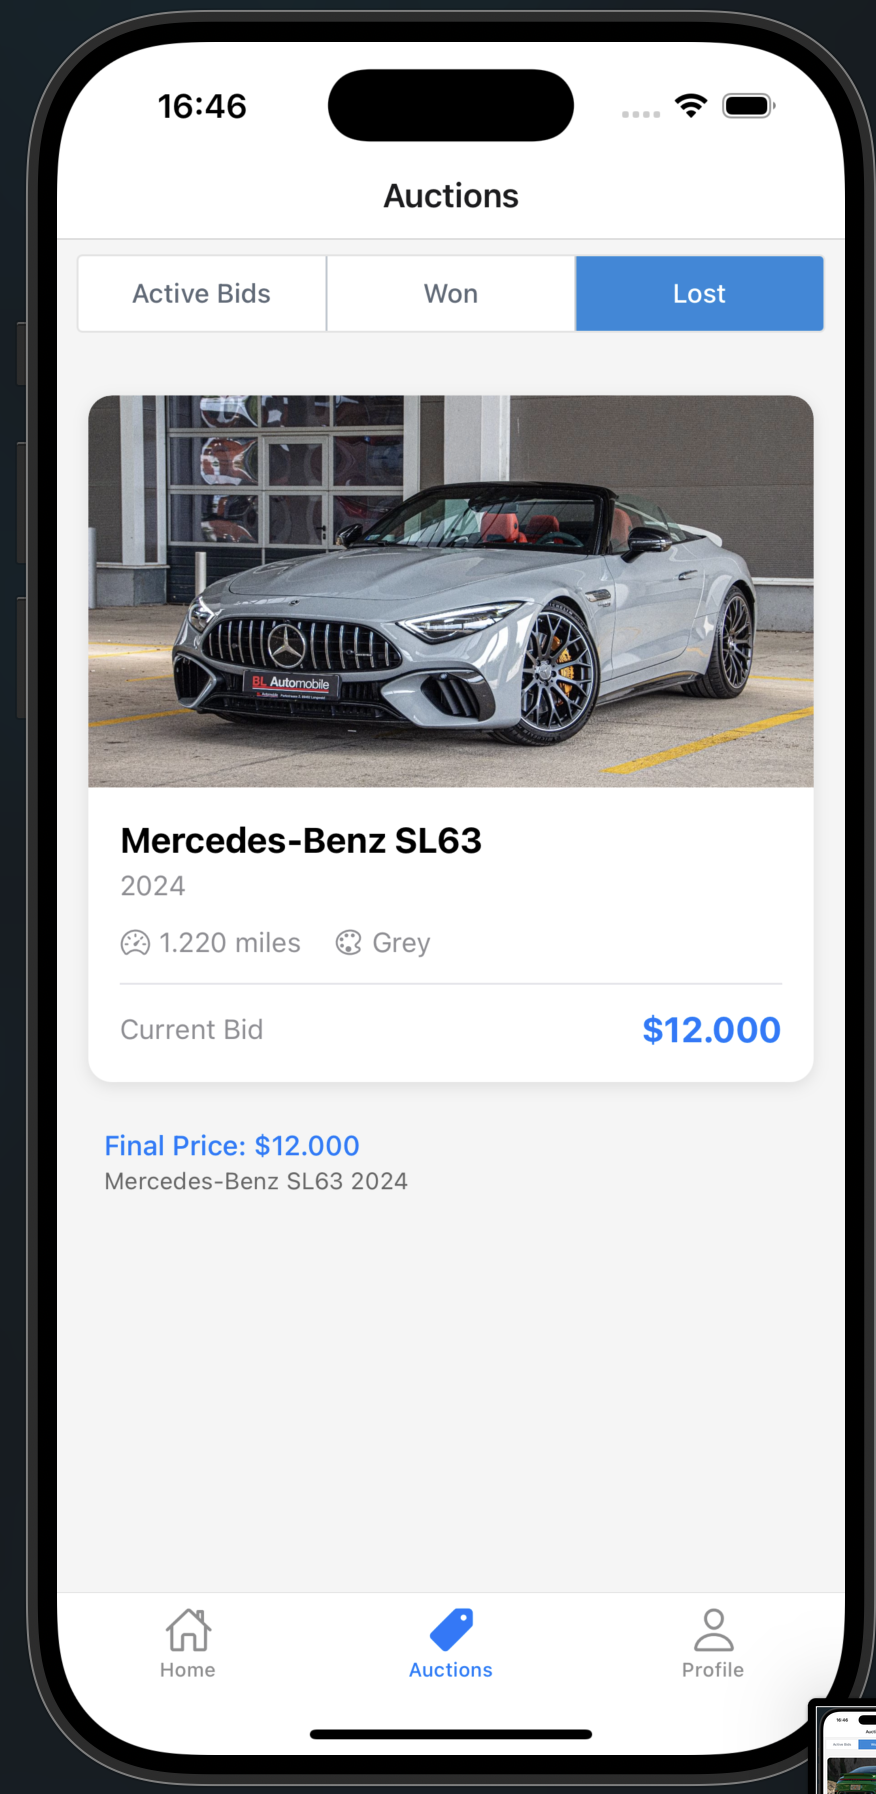
\includegraphics[width=\textwidth]{images/auction page with lost bids.png}
        \caption{Enchères perdues}
        \label{fig:lost-auctions}
    \end{subfigure}
    \caption{Écrans de gestion des enchères}
    \label{fig:auction-management}
\end{figure}

Les utilisateurs peuvent suivre leurs enchères via différents onglets : enchères actives (Figure \ref{fig:active-bids}), enchères gagnées (Figure \ref{fig:won-auctions}) et enchères perdues (Figure \ref{fig:lost-auctions}).

\subsection{Profil Utilisateur}

\begin{figure}[H]
    \centering
    \begin{subfigure}[b]{0.48\textwidth}
        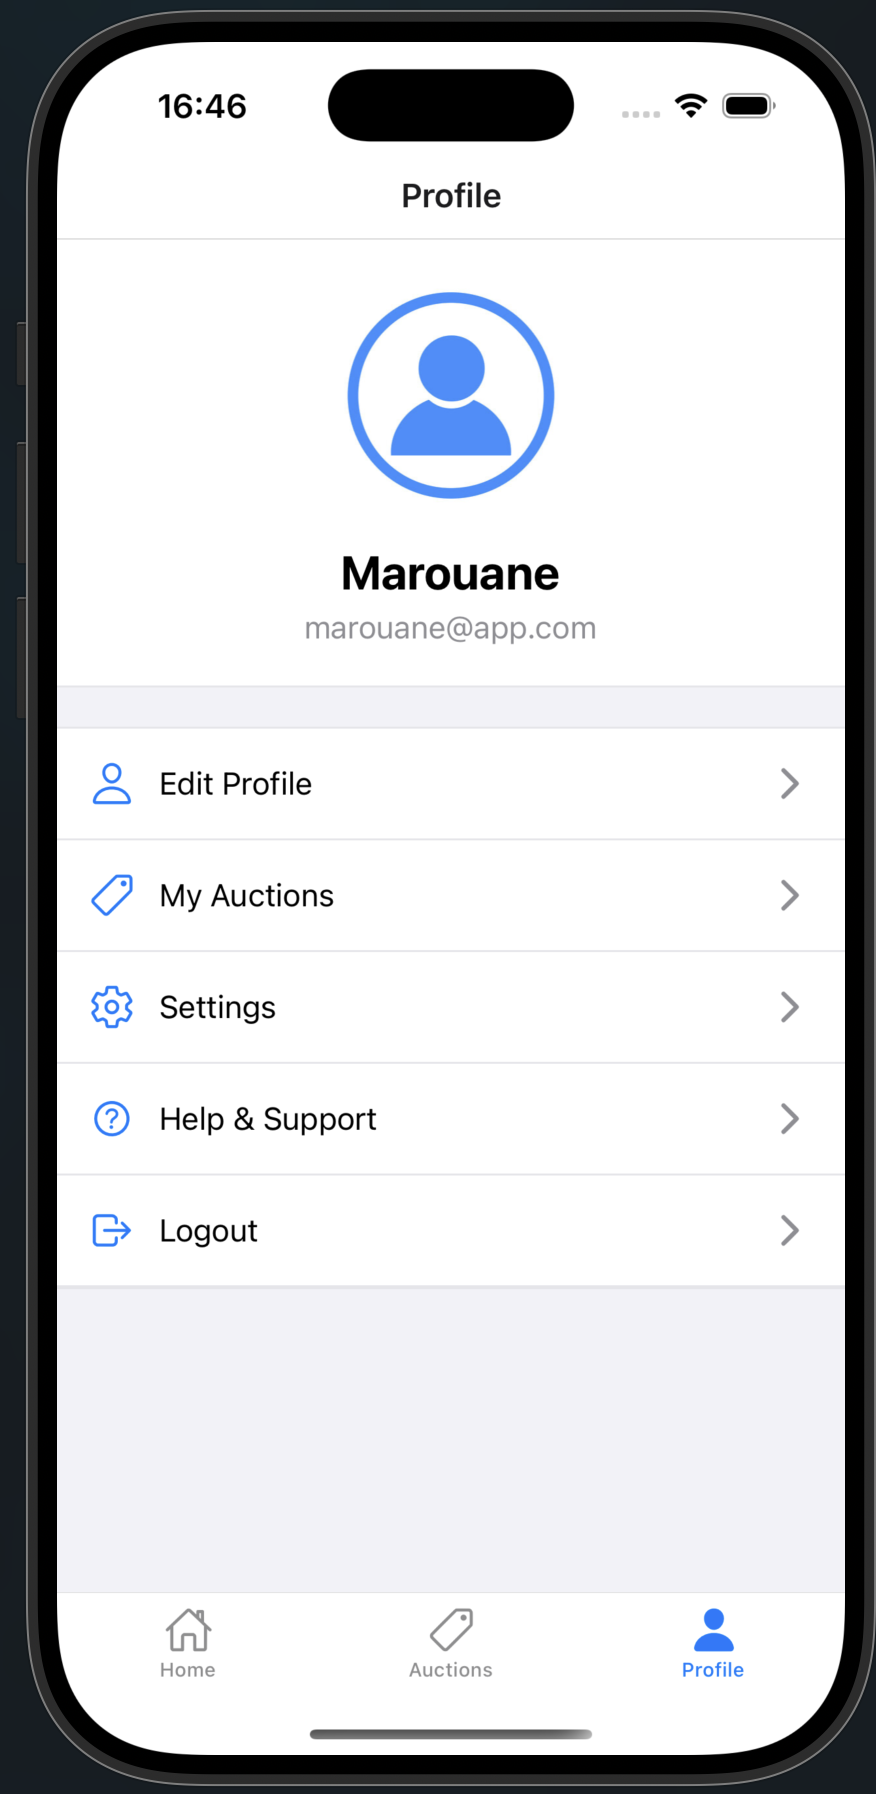
\includegraphics[width=\textwidth]{images/profile screen.png}
        \caption{Écran de profil}
        \label{fig:profile}
    \end{subfigure}
    \hfill
    \begin{subfigure}[b]{0.48\textwidth}
        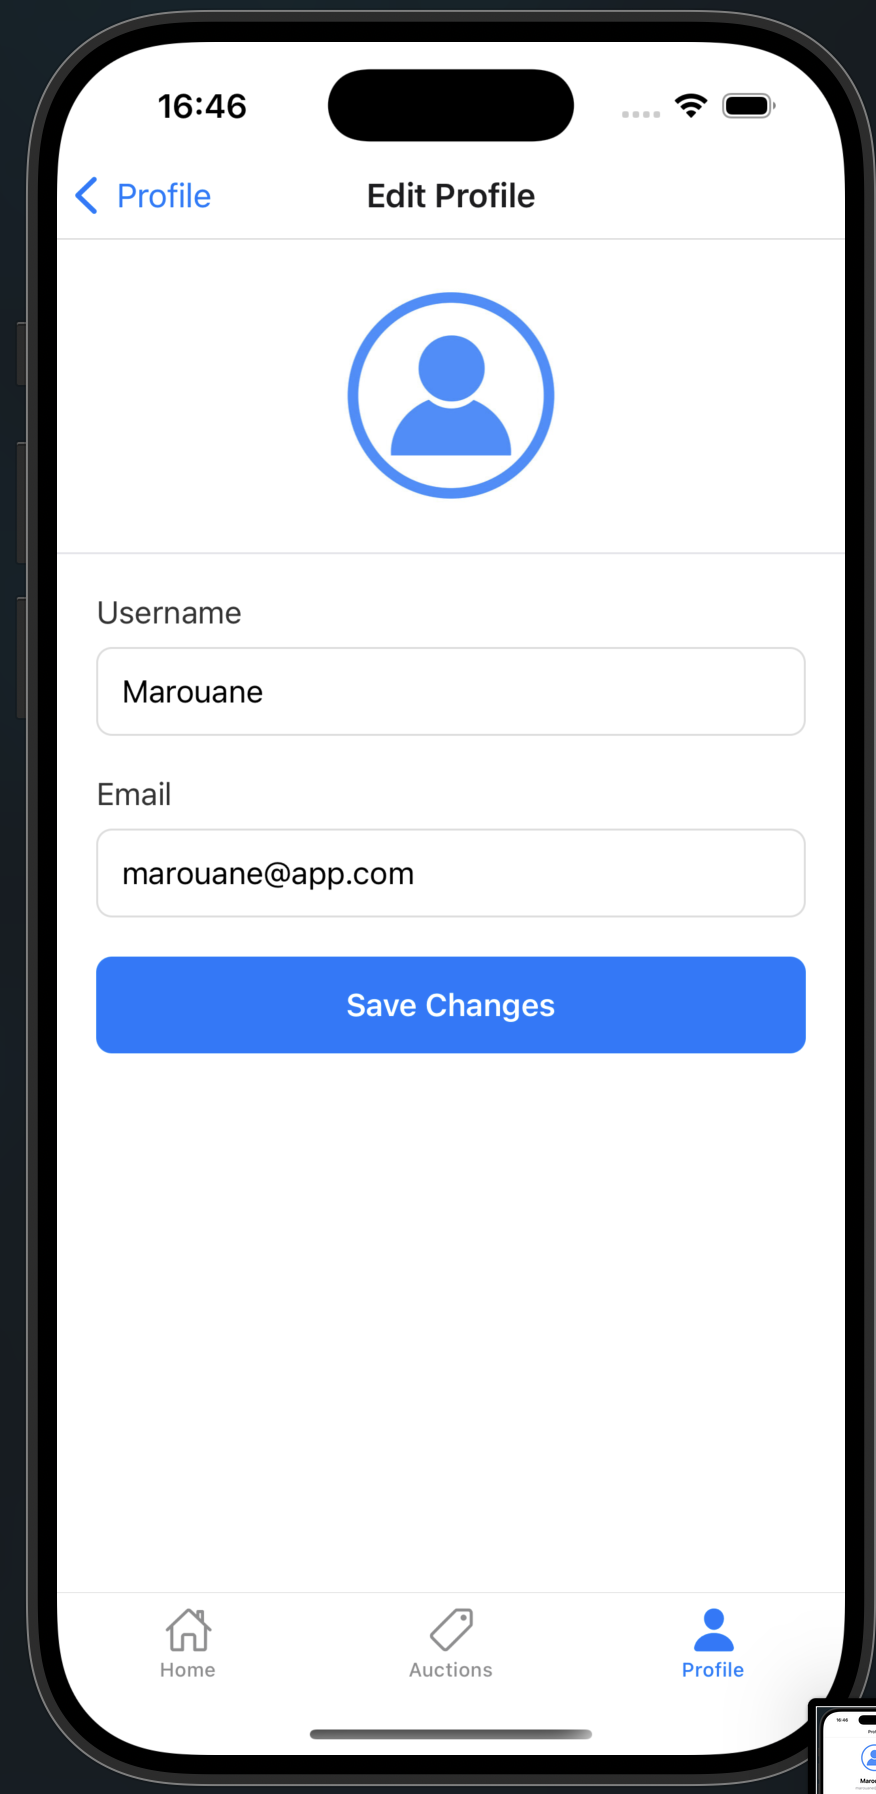
\includegraphics[width=\textwidth]{images/profile edit .png}
        \caption{Modification du profil}
        \label{fig:profile-edit}
    \end{subfigure}
    \caption{Gestion du profil utilisateur}
    \label{fig:profile-management}
\end{figure}

L'écran de profil (Figure \ref{fig:profile}) permet d'accéder aux informations personnelles de l'utilisateur et à l'historique de ses enchères. L'écran de modification du profil (Figure \ref{fig:profile-edit}) permet de mettre à jour les informations personnelles.

\subsection{Détails du Véhicule et Enchère}

\begin{figure}[H]
    \centering
    \begin{subfigure}[b]{0.48\textwidth}
        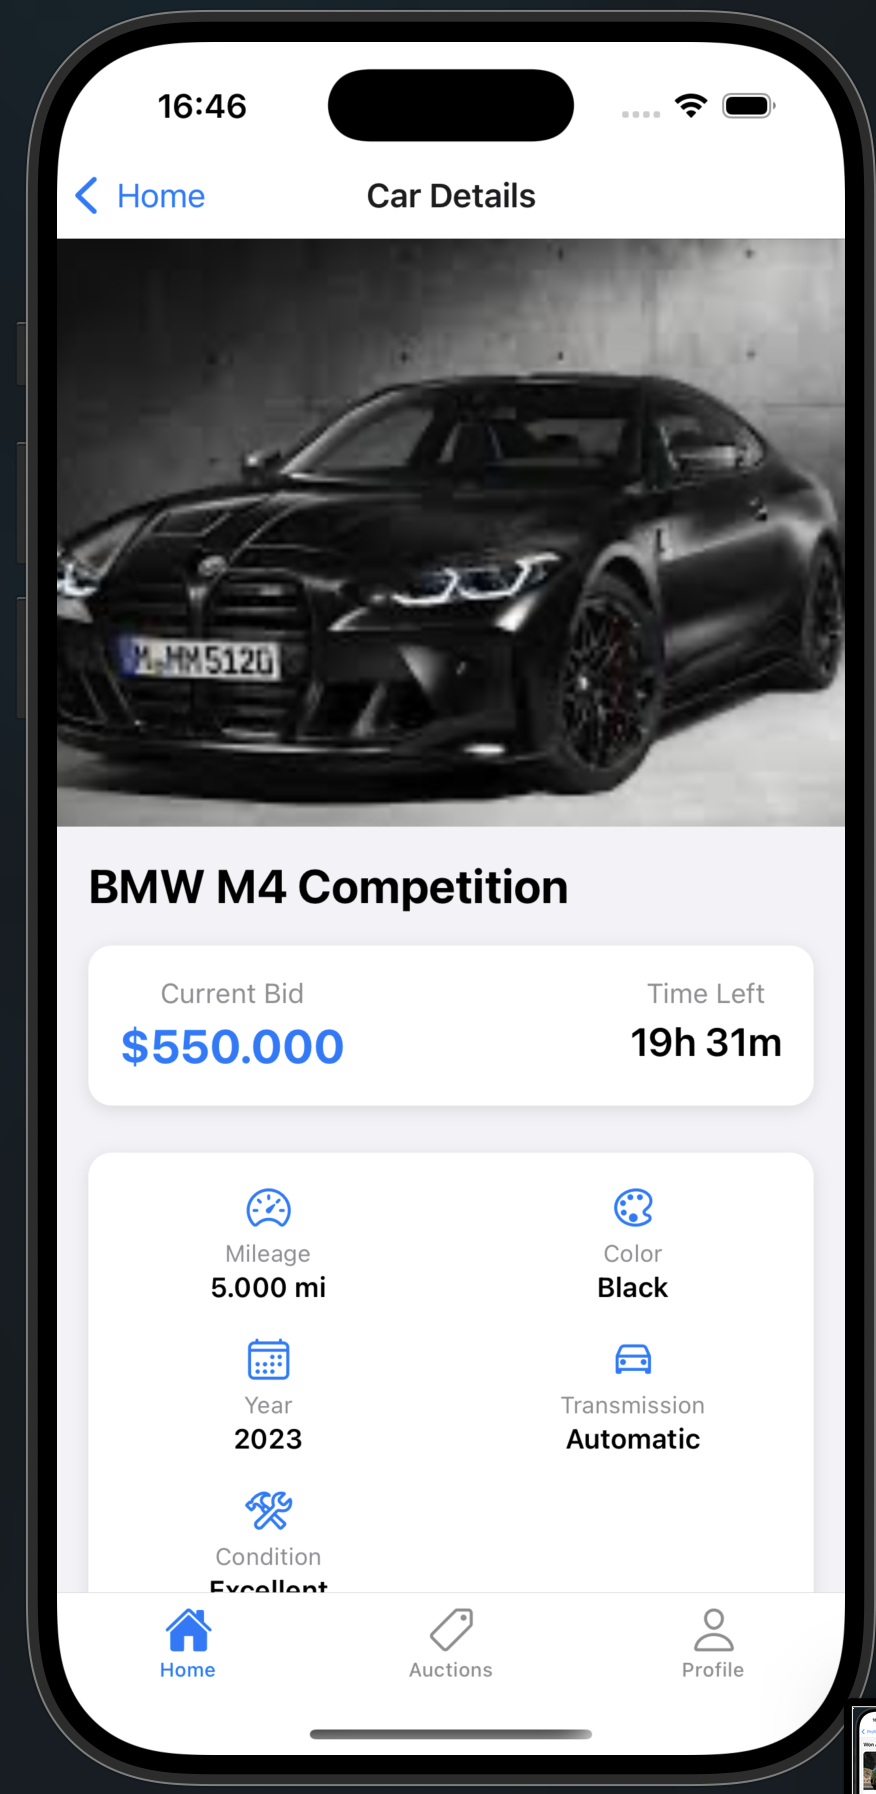
\includegraphics[width=\textwidth]{images/auction details 1 .png}
        \caption{Informations du véhicule}
        \label{fig:car-details1}
    \end{subfigure}
    \hfill
    \begin{subfigure}[b]{0.48\textwidth}
        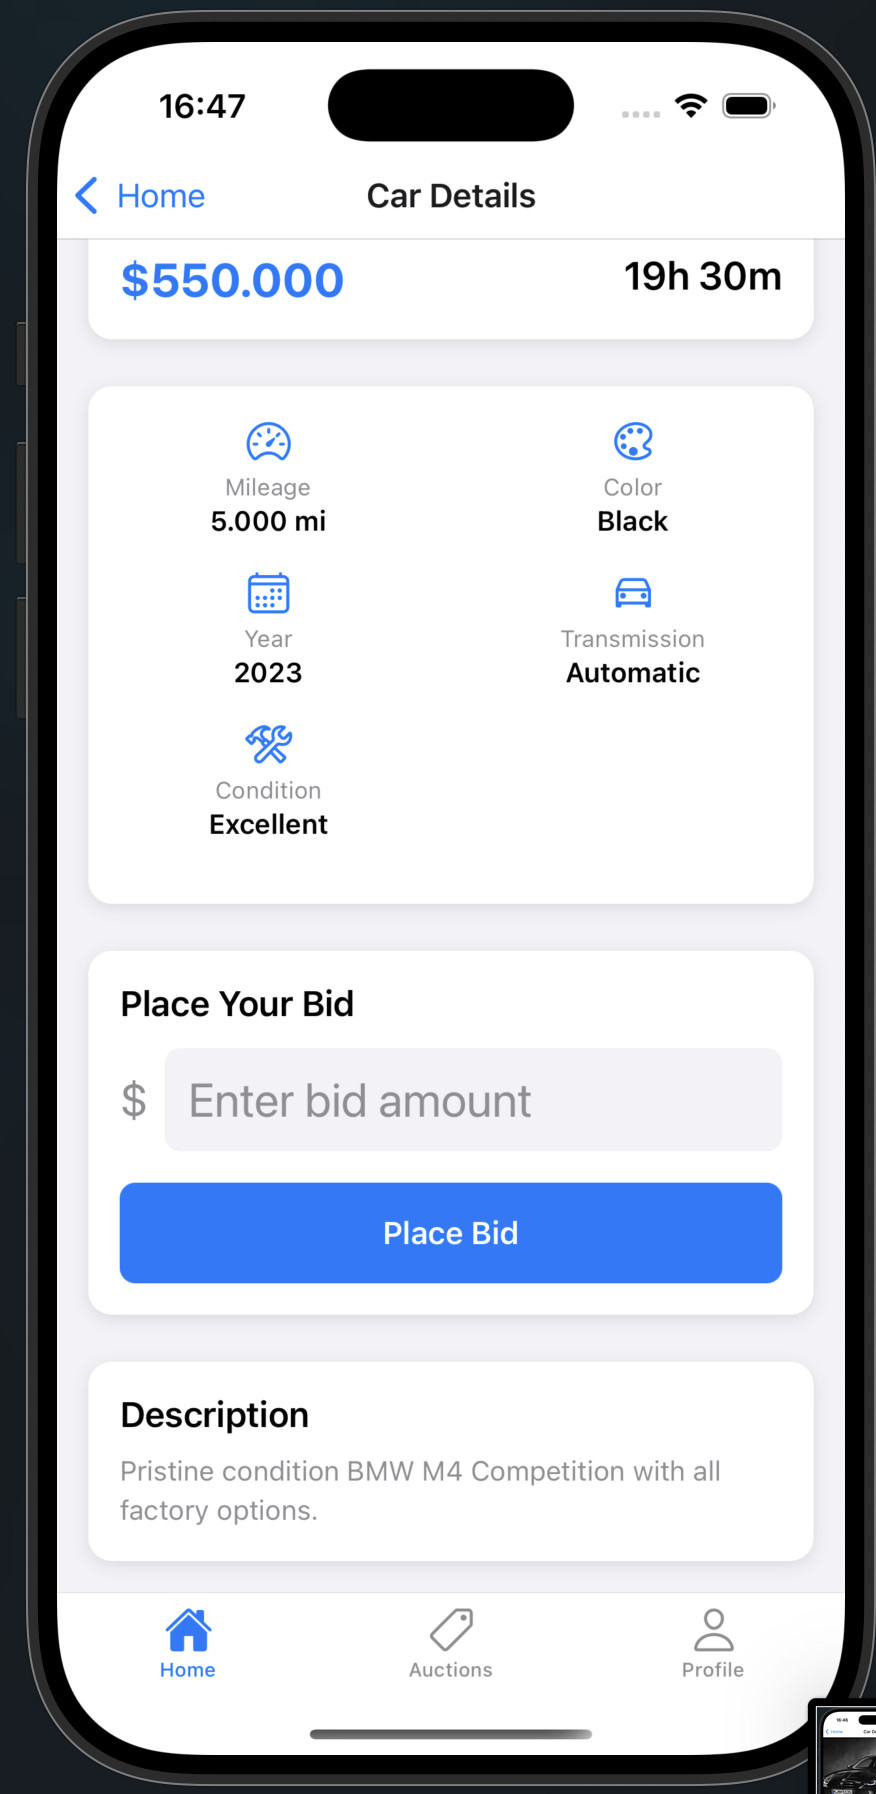
\includegraphics[width=\textwidth]{images/auction details 2.png}
        \caption{Placement d'enchère}
        \label{fig:car-details2}
    \end{subfigure}
    \caption{Détails du véhicule et système d'enchères}
    \label{fig:car-details}
\end{figure}

Les écrans de détails du véhicule (Figures \ref{fig:car-details1} et \ref{fig:car-details2}) présentent toutes les informations pertinentes sur le véhicule et permettent de placer une enchère directement depuis l'application.

\subsection{Historique des Enchères}

\begin{figure}[H]
    \centering
    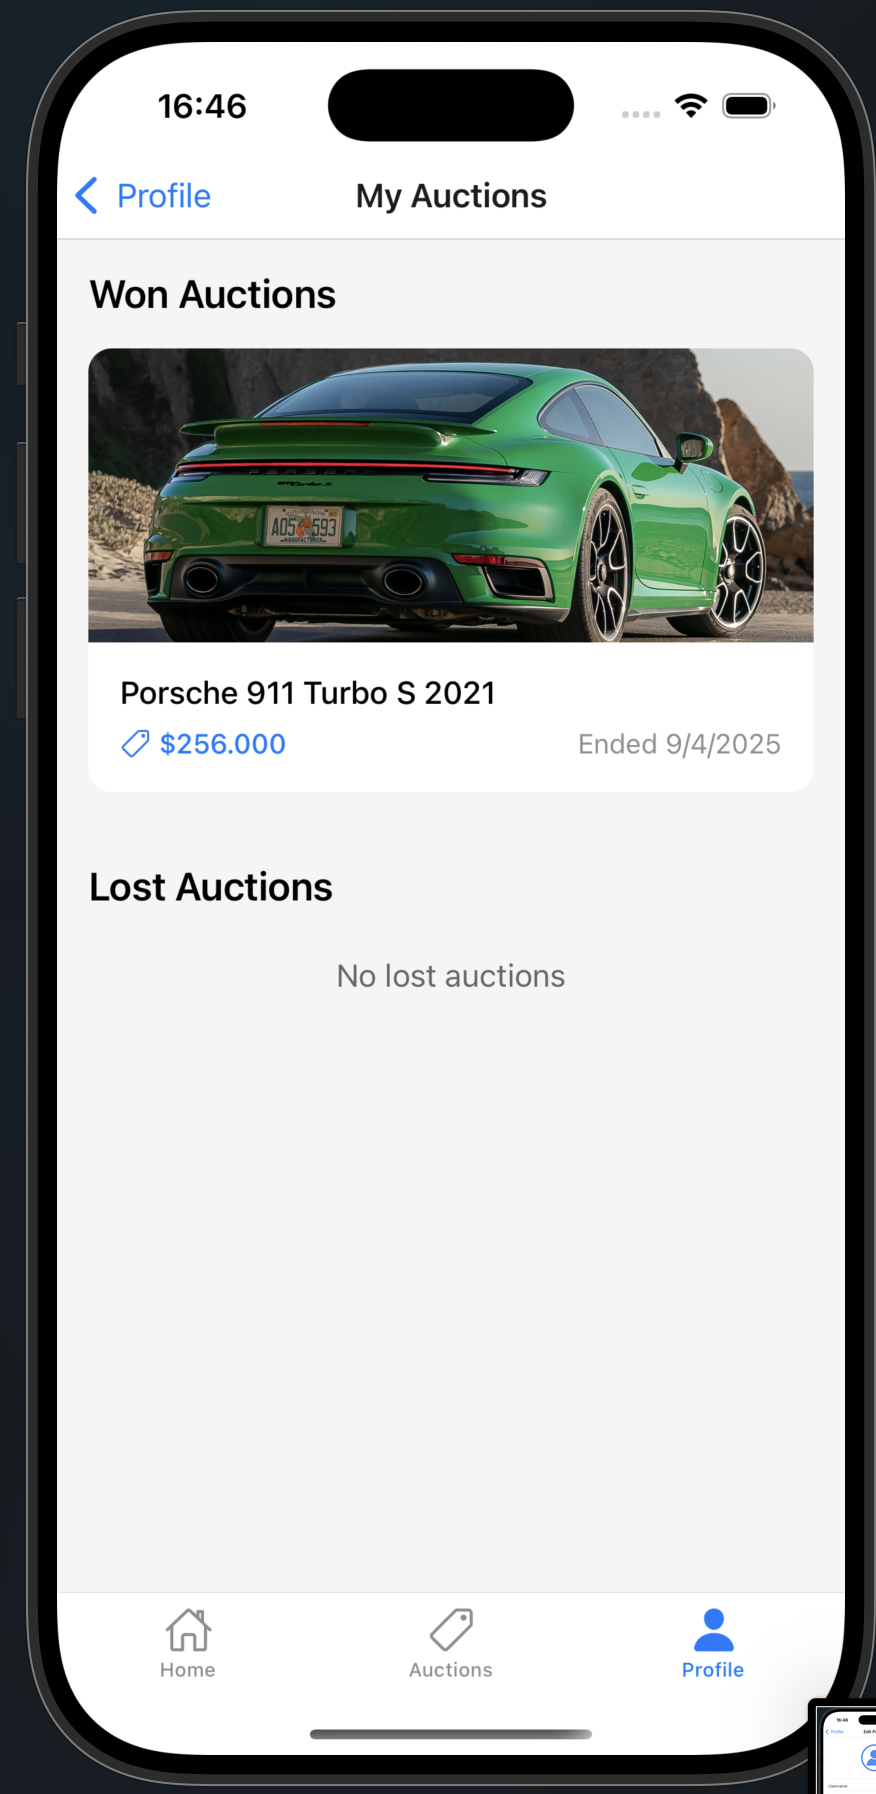
\includegraphics[width=0.6\textwidth]{images/auctions history.png}
    \caption{Historique des enchères de l'utilisateur}
    \label{fig:auction-history}
\end{figure}

L'écran d'historique des enchères (Figure \ref{fig:auction-history}) permet à l'utilisateur de consulter l'ensemble de ses activités d'enchères passées, incluant les véhicules sur lesquels il a enchéri, les montants proposés et les résultats obtenus.

\section{Fonctionnalités Principales}

\begin{itemize}
    \item \textbf{Inscription et connexion} : Création de compte et authentification sécurisée
    \item \textbf{Navigation des enchères} : Parcourir les enchères en cours et à venir
    \item \textbf{Participation aux enchères} : Placer des enchères sur les véhicules désirés
    \item \textbf{Suivi des enchères} : Consulter l'état de vos enchères actives, gagnées et perdues
    \item \textbf{Gestion du profil} : Mettre à jour vos informations personnelles
    \item \textbf{Notifications} : Recevoir des alertes en temps réel sur les enchères suivies
\end{itemize}

\section{Conseils d'Utilisation}

\begin{itemize}
    \item Configurez les notifications pour être informé des changements d'enchères
    \item Vérifiez régulièrement l'onglet "Enchères actives" pour suivre vos enchères en cours
    \item Complétez intégralement votre profil pour faciliter les transactions
    \item Consultez les détails complets du véhicule avant de placer une enchère
    \item Définissez un budget maximum pour chaque enchère pour éviter les dépassements
\end{itemize} 